%*******************************************************************************
%****************************** Fifth Chapter *********************************
%*******************************************************************************

\chapter{Image processing results and discussion}

\ifpdf
    \graphicspath{{Chapter5/Figs/Raster/}{Chapter5/Figs/PDF/}{Chapter5/Figs/}}
\else
    \graphicspath{{Chapter5/Figs/Vector/}{Chapter5/Figs/}}
\fi

%********************************** %First Section  **************************************
\section{Introduction}

To compare this method with previous work, the images generated were evaluated based on their use in segmentation as compared with a manually segmented subset of the data. The methods, Selinummi, Maximum GFP, and the current method, can be compared under similar conditions using the same dataset. A readily available property of the cell instances found is the projected cell area. Other properties are the number and orientation of the cell protrusions. These will also be compared to judge the difference between the methods. An example of the comparison between the original brightfield and the final zBF image can be seen in Figure~\ref{fig:zbfcomparison}.

\begin{figure}[h!]
 \centering
 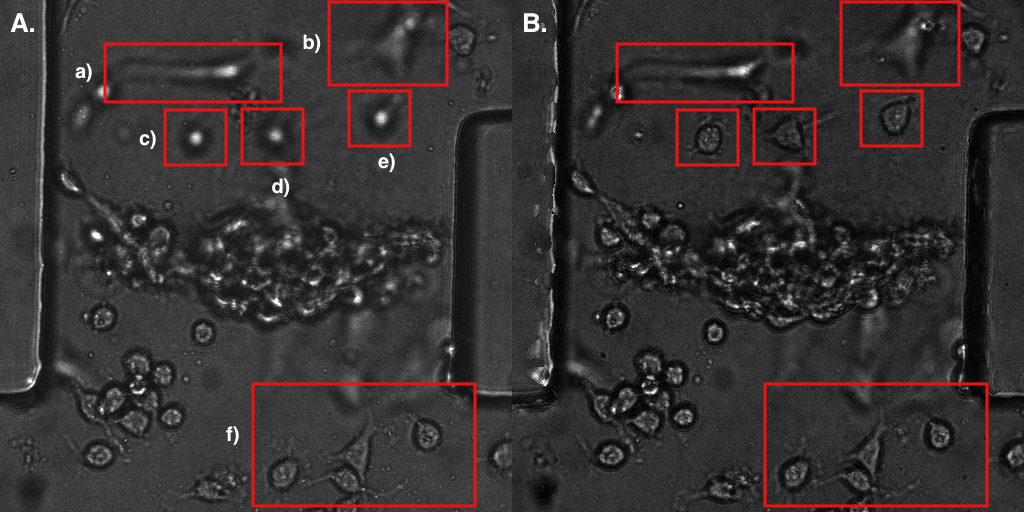
\includegraphics[width=0.9\textwidth]{501_zbf_comparison}
 \caption[zBF comparison with brightfield]{
 	This is a side-by-side comparison of the zBF modification with a single slice of the original brightfield data. The changes that have been made are mostly the adjustment of focus in the appearance of cells that are marked with GFP. Note first of all that cells a) and b) have not been adjusted. These are not marked with GFP and are not affected by any of the algorithms. Cells c), d), and e) originally appear to be out of focus in image A, but in B, they appear in focus. This is part of the correction made. The cells in group f) have been adjusted, but their corrections lie much closer to the focus they originally occupied in this slice. They still appear in focus. All cells marked with GFP have been level corrected. This is the most powerful result of this study.
 }
 \label{fig:zbfcomparison}
\end{figure}

Despite the improvements made, the method developed is not without error. There are parameters that have optimal ranges, but outside those ranges, the method can fail. Some physical properties of the environment can limit the effectiveness of the method, for example, if the level of the GFP is too low to generate an accurate estimate of the Z level, the focus of GFP marked objects will not be corrected accurately, and the results will not be useful. Additionally, some configurations of cells in close proximity can cause problems for this method. A clear example is when two cell lie vertically one on top of the other, causing two visible peaks in the GFP. This, and other examples are discussed in Chapter 4.

A common problem when comparing methods of the segmentation is that there is no objective ``ground truth", or definitely correct answer to the question of the shape parameters of the objects of interest. In their paper, Selinummi et al. attempted to define the ground truth as the segmented shape from the GFP projection~\cite{Selinummi:09}. This method is a poor representation of the cell and is prone to errors. For this reason, the ground truth chosen for the comparison of the methods shown here is the manual segmentation, or outlines of the cells drawn by eye on the zBF image. Only of sample of the frames are considered since manual segmentation is very time consuming. Yet another problem, is that not even the manual segmentation can be considered the ground truth. The human eye cannot be trusted to determine the shape of an object which it is totally unfit to identify in an environment that does not lend itself to casual observation. Despite this obstructing piece of philosophy, the final judgement must lie with something, and the best thing available is human vision, which is not saying much in the microscopic world. We are left with no choice but to accept a system of pattern recognition whose highest reccommendation is that it insists on discovering human faces wherever it looks~\cite{Fyfe:08}.

\section{Parameter sensativity study: $R$, $\Delta Z$, $\Sigma$}

The three parameters that contribute to the generation of zBF must be carefully chosen, since a low quality result will be useless for segmentation. An analysis of the sensativity of the result to changes in the parameters can be used to determine the optimum values. Below, some examples of parameters chosen outside the optimal ranges are shown and some consequences of their segmentation is investigated.

\subsection{The radius of GFP linear smoothing: $R$}

The parameter $R$ is the radius of the linear smoothing filter applied to the GFP in order to generate a profile for a point in XY. The filter mixes values in XY, but not Z. It has the effect of reducing noise and making transitions between levels of neighbouring pixels more fluid. This helps to reduce the problem of cross-level artifacts, discussed in Section~\ref{sec:errors}. In the case where neighbouring objects in XY has very different levels in Z, the level transition would be smoothed such that the point half way between them would be assigned to a level half way in Z. While this case has not been observed, it could lead to strange results, such as half of each cell being in focus, while the halves closest to the other cell are out of focus. This would depend on the radius of the linear filter, but at a certain point, the information is too smoothed and ceases to be useful. Below in Figure~\ref{fig:rvariation} is an example of the linear filter set too high. The logical limit is a smoothing filter the size of the image itself in XY. This would simply yield the sum or mean of the GFP for each focal plane, which would not provide any more information than where most of the cells were found in the environment.

On the other hand, if the size of the linear filter is too low, such as a single pixel, the noise in the GFP would dominate the Z estimate, leading to highly fluctuating Z values across even a single cell. The result in the zBF image is an extremely noisy cell interior and edge, surrounded by an equally noisy background. This does not lend itself to accurate segmentation. Figure~\ref{fig:rvariation} is an example of the linear filter using a small $R$.

\begin{figure}[h!]
 \centering
 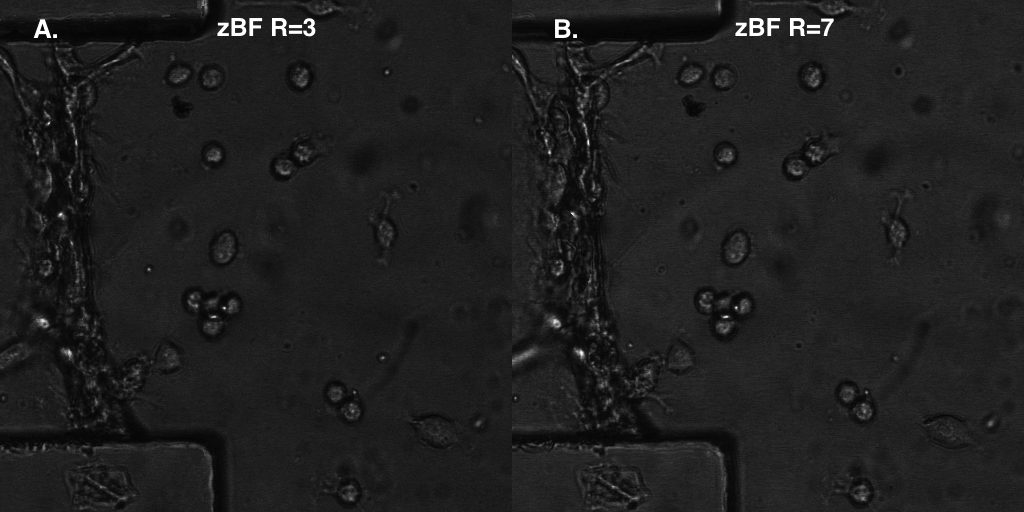
\includegraphics[width=0.9\textwidth]{502_r_variation}
 \caption[Varying R]{
 	This is an example of the variation of the parameter R, or the linear smoothing kernel that operates in 2D in the GFP. A shows the zBF image with $R=3$. B shows $R=7$. Note no brightfield information has been smoothed. Brightfield information is accepted or rejected by decisions made using the GFP. Consequently, the parameter R does not have much of an effect on the zBF image. It can be set to a constant value. That is neither 0, such that noise is not preserved, nor proportional to the size of the image, such that information about features is not destroyed. If the Gaussian kernel were set to the size of the image, this would be equivalent to setting the value of each pixel in the zBF image to the value of the brightfield pixel at the mean Z at which GFP is found.
 }
 \label{fig:rvariation}
\end{figure}

\subsection{The brightfield level correction: $\Delta Z$}

The weakest part of the method is the spatial relationship between the brightfield and the GFP and the decision about the value of $\Delta Z$. The brightfield is subject to fluctuations from the autofocus and has no intrinsic spatial information. The most important piece of information relating the GFP and the brightfield is for a hypothetical fixed object in focus in the brightfield, the GFP representation will always correspond to that level of focus. This is because the position of the microscope hardware is constant for a single frame and is set by the autofocus estimate from the brightfield. Assuming the same physical space is represented in both, the GFP can be used to account for the autofocus fluctuations, but the relationship between the GFP representation and the appearance of an object in the brightfield is arbitrary. A cell may be ``in focus" as far as possible, but still not be clearly visible by a human. This hinders manual tracking. optimum features for observation may not correspond to optimum features for segmentation. For tracking, it most effective to observe an object in a solid colour with or without clear edges since the precise shape is not necessary to indicate object centres. For segmentation, a clear object boundary with dark edges and a smooth, uniformally coloured interior yields the most accurate shape. This discrepancy is represented by the empirically determined value, delta-Z. Changing this value results in what would normally be seen as focussing a simple lens looking at a 2D environment. This effect can be seen in Figure~\ref{fig:deltazvariation}. Through further study, a value could be found automatically, but the focus level for optimum human observation is highly subjective.

\begin{figure}[h!]
 \centering
 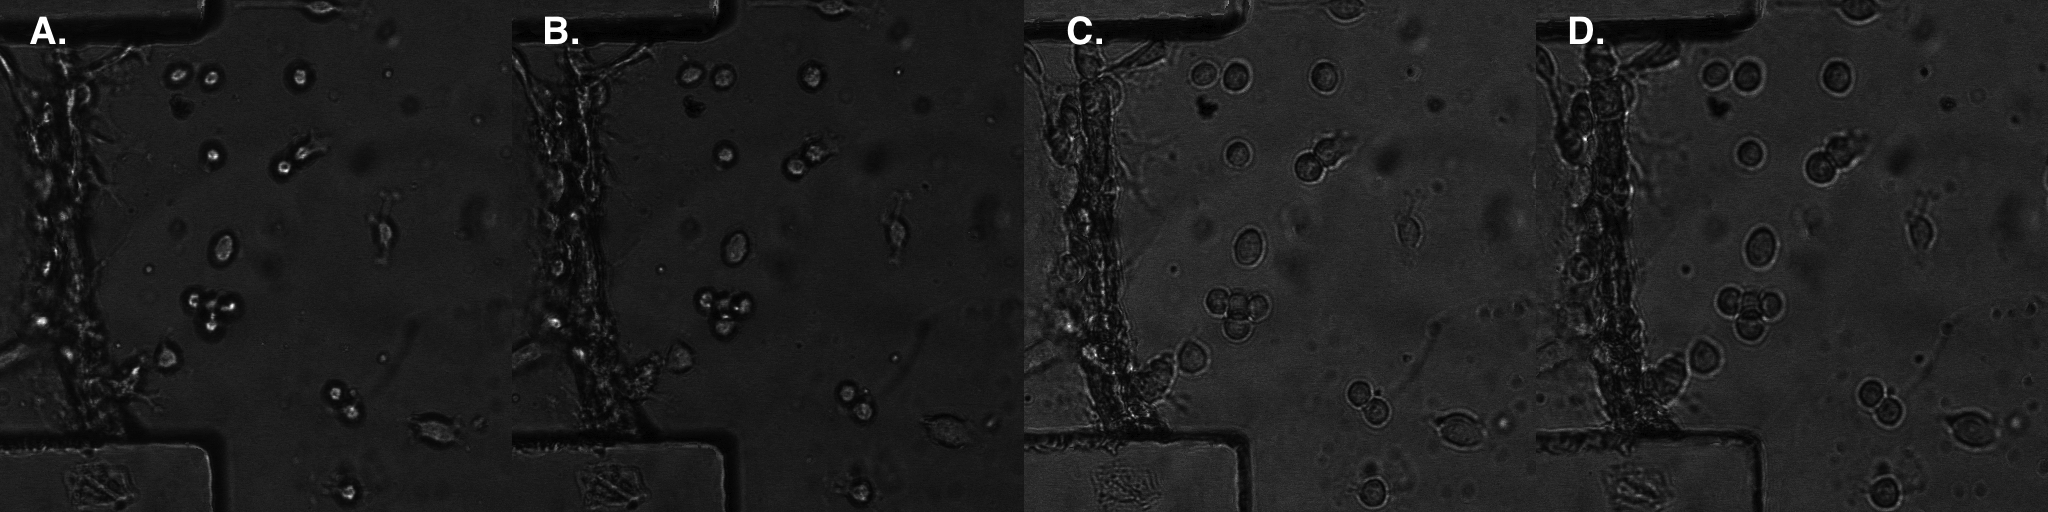
\includegraphics[width=0.9\textwidth]{503_deltaz_variation}
 \caption[Varying $\Delta Z$]{
 	The value of $\Delta Z$ is very important to the final appearance of the zBF image, shown in A, B, C, D, but must be determined empiracally, or by a trusted, previously determined algorithm. It is the level offset between the location of the GFP representations of cells and their brightfield counterparts. Changing $\Delta Z$ is equivalent to focussing a microscope objective that is looking at a 2D slide or other simple environment. Focussing too far in one direction will have the effect of leaving every corrected object in the environment out of focus.
 }
 \label{fig:deltazvariation}
\end{figure}

\subsection{The radius of level Gaussian blur: $\Sigma$}

The radius of the Gaussian blur between levels, or $\Sigma$, affects how smooth the transitions between levels are in the GFP. It mixes data from different parts of the environment in 3D. This does not affect the output in the brightfield greatly, but it can prevent errors. An example of the variation can be seen in Figure~\ref{fig:sigmavariation}, and the results of the ignoring this parameter can be seen in Figure~\ref{fig:crosslevelartefacts}.

\begin{figure}[h!]
 \centering
 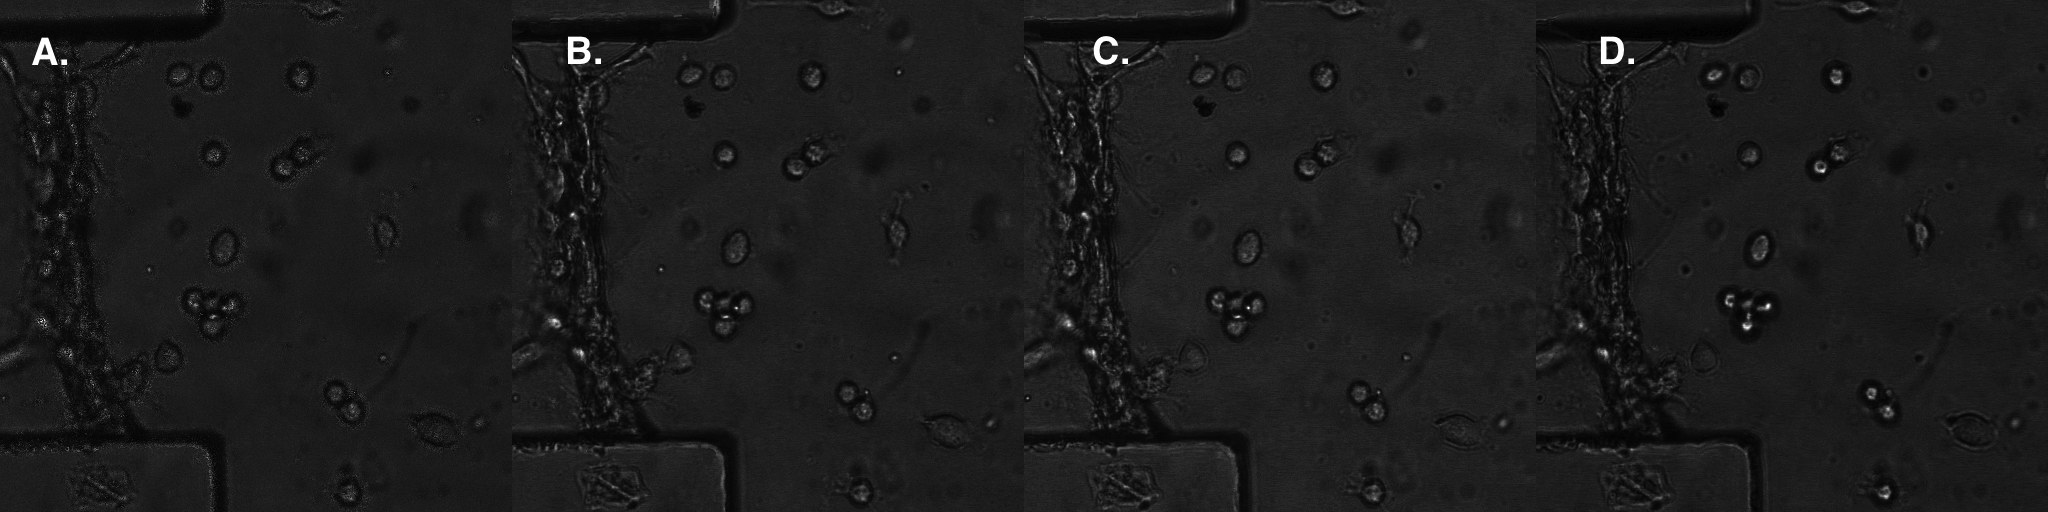
\includegraphics[width=0.9\textwidth]{504_sigma_variation}
 \caption[Varying $\Sigma$]{
 	$\Sigma$ is a very important parameter that affects the smoothing of the GFP in 3D. If it is set too high, features can be destroyed very easily. A reasonable value can prevent noise dominating the level corrections. The best example of dominant noise is the image in A. Even though the brightfield is not affected by the GFP processing, the noise in the GFP leads to a very noisy appearance in the values chosen from the brightfield.
 }
 \label{fig:sigmavariation}
\end{figure}

\subsection{Final choice of parameters}

The three variables used to produce zBF were fixed to the following values. These were also chosen for their effects on zUnique and zEdge:

\begin{center}
	\begin{tabular}{ | l | p{5cm} | l | p{5cm} |}
		\hline
		Parameter & Description & Chosen range & Reason \\ \hline
		R & Radius of 2D linear smoothing kernel in XY & 3-5 pixels & Reduce noise in GFP images. \\ \hline
		$\Delta z$ & Difference between observed in-focus level and optimal edges for segmentation & -6 to -8 levels & Determined by observation and segmentation testing. \\ \hline
		$\Sigma$ & Radius of 3D Gaussian smoothing kernel & 5-7 pixels & Make transitions between regions with similar Z more gradual to prevent cross-level artefacts. See Figure~\ref{fig:crosslevelartefacts}. \\ \hline
	\end{tabular}
\end{center}

\subsection{The subject of the background}

It should be noted that background pixels in XY that contain very little GFP at any Z, and thus have very flat profiles, are still assigned a value for the Z position. This may appear misleading, as it can be highly random as the ``maximum" of a flat distribution is given by the noise alone. This can be seen clearly in the PDMS pillars in Figure~\ref{fig:falsezvariation}, indicated by an arrow. While this might be thought to produce errors, other means of filtering background can be used that do not rely on the Z position, such as the mean image. It is more reliable to be unbiased when generating the zMod image since there is no certain way of determining whether a particular Z value should be assigned. If filtering must be done eventually, it can be done using other 3D data.

\subsection{Subsequent effects on zUnique and zEdge}

The three parameters discussed here can also affect the zUnique and zEdge images in specific ways. Zunique is based solely on the GFP information, so cannot be affected by $\Delta Z$, but $\Sigma$ and $R$ will affect the smoothing of the zUnique information. Smoothing the GFP will spread the information and the Z placement of the maximum intensity in neighbouring pixels. This could cause the mask of the segmentation of the zUnique image to appear larger with larger $R$ and $\Sigma$. This, in turn, will affect the edges placed into the zEdge image. The edges could become thicker and further away from the mask of the cell. This could allow parts of the background surrounding the cell to be included in the final mask. The zBF component of the zEdge image will be affected by the parameters in the same way as the original zBF image.

\begin{figure}[h!]
 \centering
 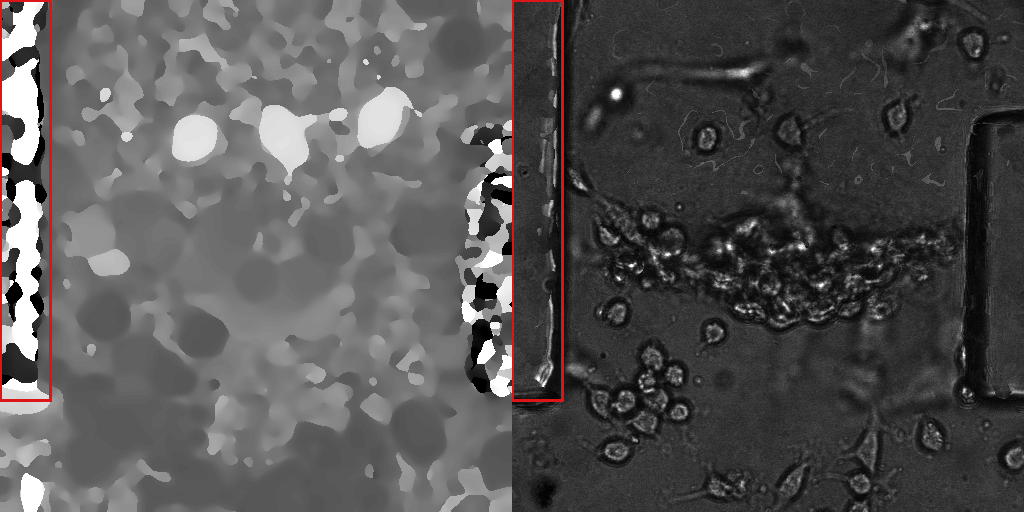
\includegraphics[width=0.9\textwidth]{505_false_variation}
 \caption[False Z variation]{
 	Even the noise and background is assigned a Z value. This seems counterintuitive when applied to the background, but the philosophy of this study is that any analysis or segmentation cannot be biased to sizes and shapes of objects. All locations in an image must be considered and treated equally until enough knowledge has been gathered and assumptions have been made to treat different areas differently. At the zMod stage, there is no certainty or assumptions about the locations or shapes of cells, so all pixels in the image are subject to the same calculations. When a profile is measured in a pixel column that contains no GFP, there will still be background noise and any slight fluctuation will yield a maximum value and its position. This value is placed in the zMod image. The rationale is that it will not affect the segmentation since these areas will be rejected as part of the background anyway. These areas are filtered out at the zVar stage which is dependent on degree of variance. These locations have no variance and will not affect the final result.
 }
 \label{fig:falsezvariation}
\end{figure}

\section{zVar and zEdge}

The zEdge image uses artifical edges to constrain the segmentation and prevent errors. The artificial dark edges are drawn on the image using the edges from the segmentation of the zUnique channel. The colour profile of the images is determined by scanning the XY brightness profile of in-focus edges in the brightfield. The quality of the edges is determined by the reliability of the segmentation of the zUnique channel, which can lead to errors. Artificial edges can cut off parts of the cell that do not contain enough GFP. An example of this effect is shown in Figure~\ref{fig:lowgfp}. If the segmentation fails completely, there will be no edge drawn. In most cases, segmentation of the brightfield in zEdge can continue as normal, although there will be no barrier to stop the segmentation from expanding. This type of effect is shown in Figure~\ref{fig:badzedge}.

\begin{figure}[h!]
 \centering
 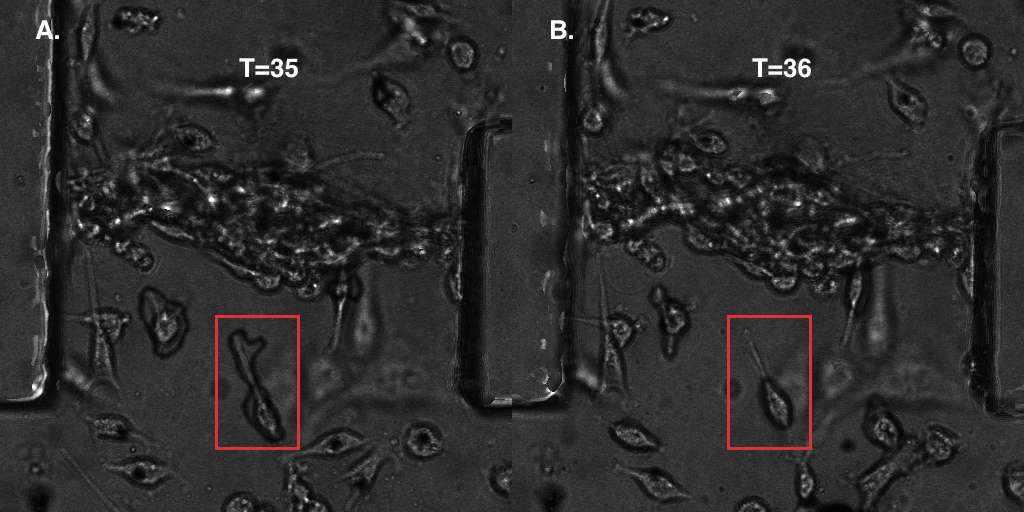
\includegraphics[width=0.9\textwidth]{506_low_gfp_edges}
 \caption[Edges in low GFP regions]{
 	One serious problem with this method is the lack of edge detection in low-contrast regions or frames in the GFP. If, due to a mechanical fault or other variation in the hardware of the microscope, the level of the GFP is lower in one frame, the method will suffer and be unable to level-correct key parts of the cell such as the protrusions. In A, the protrusion has been outlined clearly, but in B, the zEdge image has cut off the protrusion, which will prevent its segmentation. For future work, a compromise can be made between the zEdge segmentation and the unbridled zBF segmentation.
 }
 \label{fig:lowgfp}
\end{figure}

\begin{figure}[h!]
 \centering
 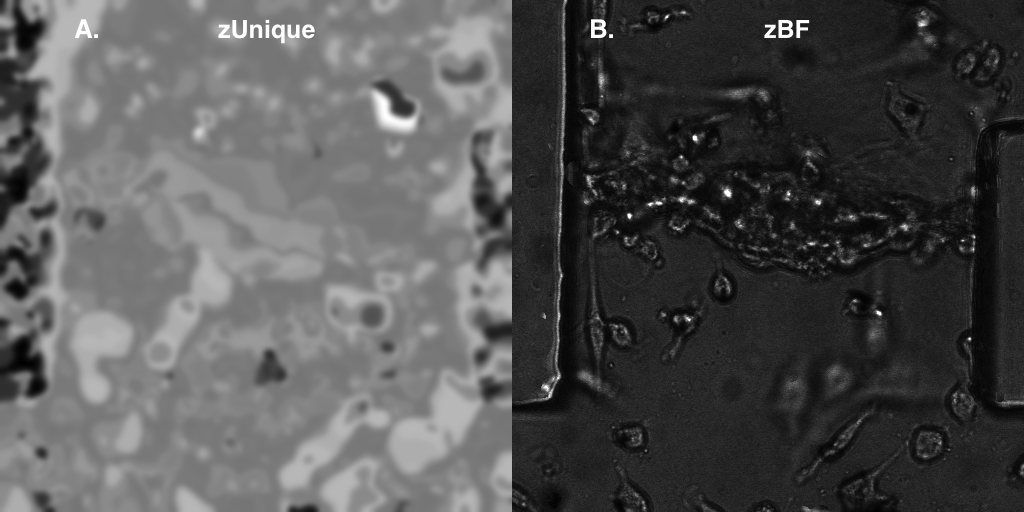
\includegraphics[width=0.9\textwidth]{507_bad_zedge}
 \caption[Ineffective zEdge]{
 	Sometimes, zUnique can yield a low-contrast image, usually, but not necessarily due to low contrast in the GFP. This can prevent the drawing of edges altogether leaving a dark spot at the position of the marker in each cell and possibly negatively affecting segmentation.
 }
 \label{fig:badzedge}
\end{figure}

\section{Comparison with common methods}

Previous methods cannot account for the inconsistencies in the focus fluctuations and so are not really comparable in their quality. Below, some of the results from segmentation of images generated using several different method including the current method. The comparisons here are based on the segmentation area, shown in Figure~\ref{fig:areacomparison} and Figure~\ref{fig:areacomparisonvalues}, although in reality, judging by the area of segmentation alone is unreliable, and an analysis of all available shape parameters should be done instead. This analysis is partially beyond the scope of this project, but leaves an opportunity for future work. Another method of comparison comes from tracking smaller cell features, such as protrusions, individually. This is also currently beyond the capabilities of the study, but current research can be easily extended to include this. A small example of how protrusions can be tracked and measured is shown in Figure~\ref{fig:protrusioncomparison}.

\begin{figure}[h!]
 \centering
 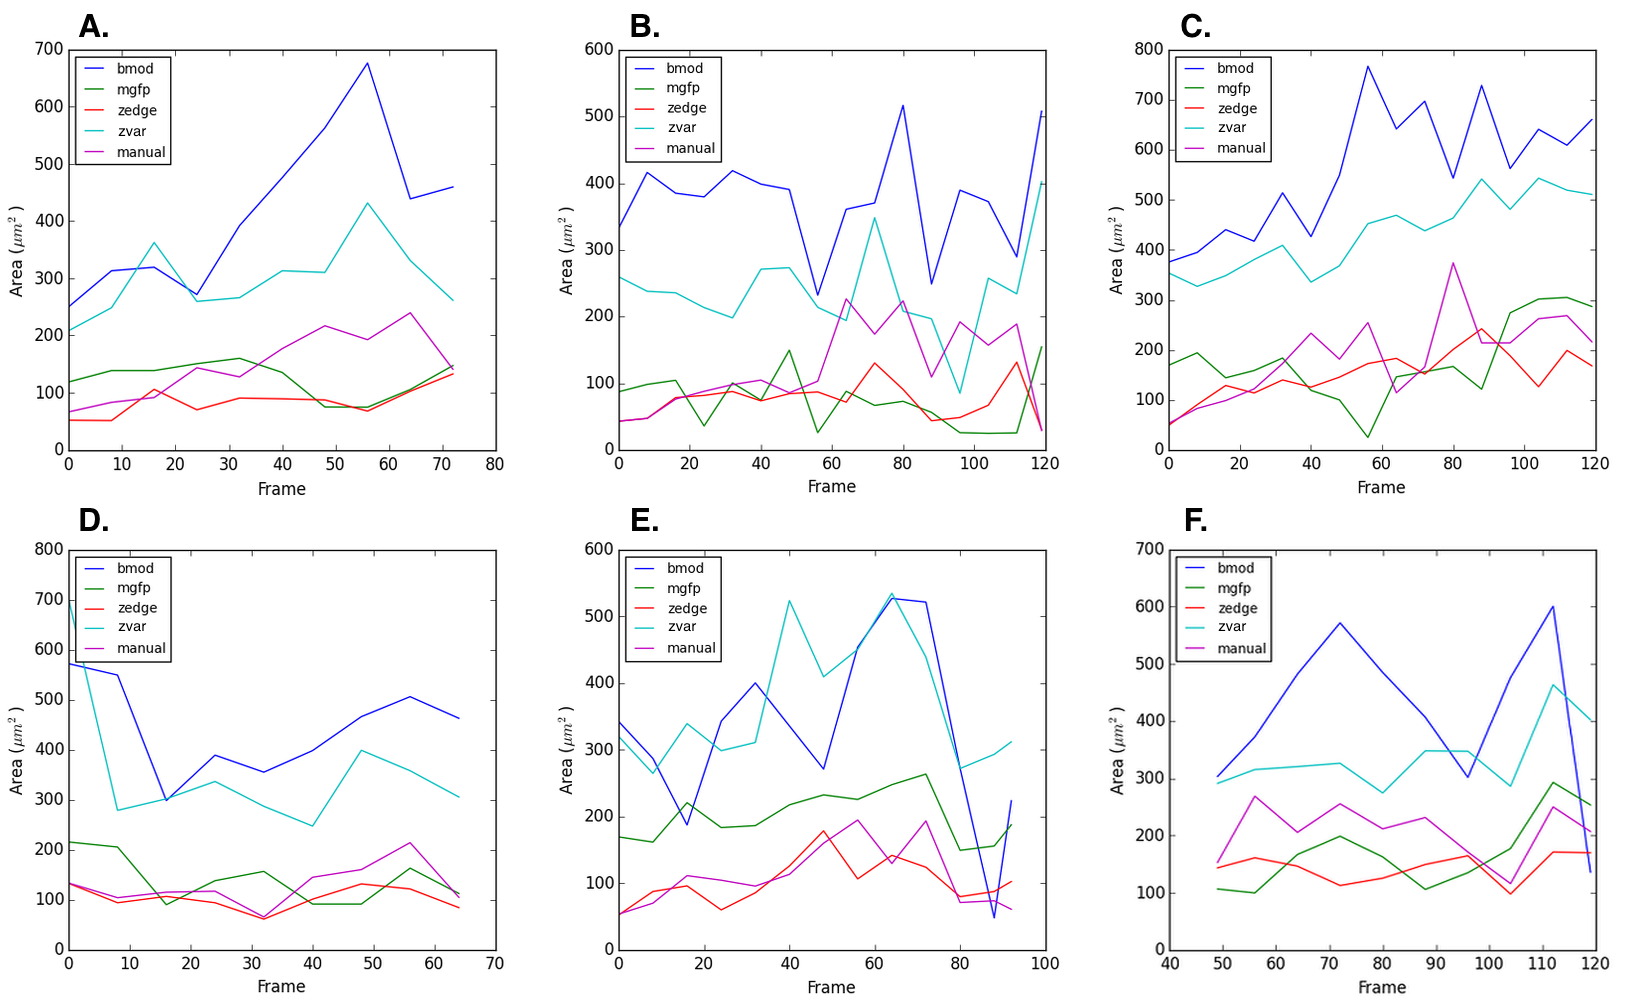
\includegraphics[width=0.9\textwidth]{508_segmentation_area_comparison}
 \caption[Testing: segmentation area comparison]{
 	In order to test the method of image modification, the best thing to be done is attempt to segment the images produced. The method of comparison used in the Selinummi paper~\cite{Selinummi:09}, which involves the comparison with the GFP projection in 3D, is insufficient to be certain about the result of segmentation. For this reason, a sample of the cells were segmented manually to provide a baseline from which to measure. Selinummi refers to this as the ``ground truth". This is shown as the purple line in each plot. The blue line is the method from the Selinummi paper. This suffers from an inability to distinguish between different types of cells and plastic, leading to an overestimate of areas as other material is incorporated into the mask from segmentation.
 }
 \label{fig:areacomparison}
\end{figure}

\begin{figure}[h!]
 \centering
 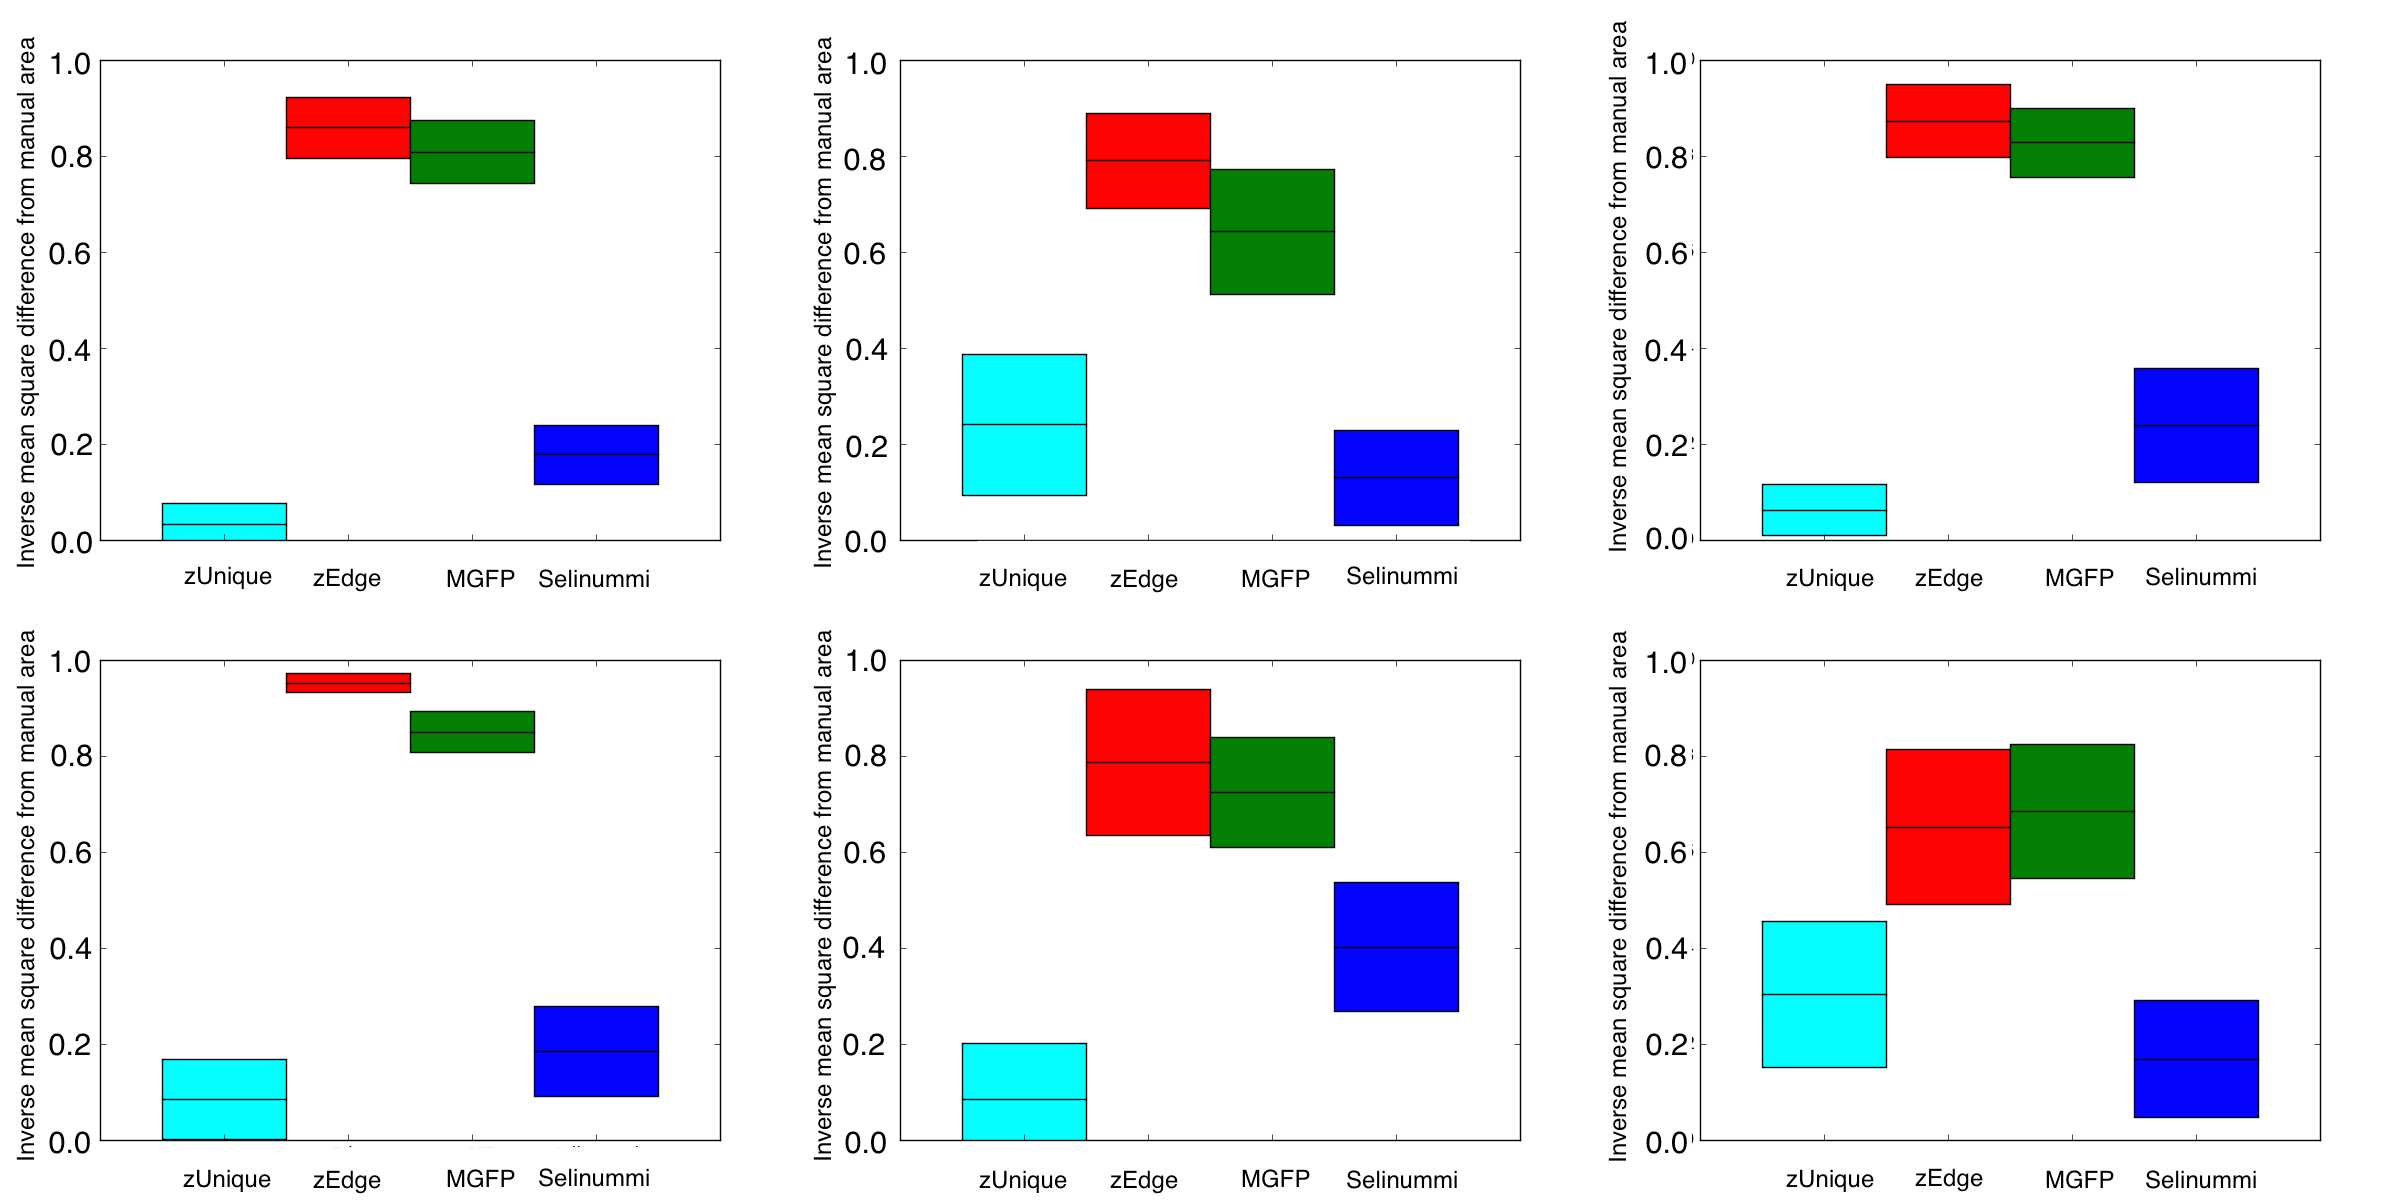
\includegraphics[width=0.9\textwidth]{509_segmentation_comparison_values}
 \caption[Testing: segmentation area comparison values]{
	Each plot shows the comparison of the segmented area of different images generated from the original image data. The first two (cyan and red) show the intermediate stage, zVar, and the final stage of the current processing method, zEdge. The last two (green and blue) show the maximum projection of the GFP and the Selinummi method respectively. A high score on the y-axis shows a better match to the manually segmented test data. The boxes show the mean (central black line) and variance (coloured box) of time series data for each cell mask. The mean and variance values for a single channel are generated by comparing the area of each mask per frame to the manually drawn mask. This series of differences is then normalised to the maximum difference from all channels at each frame. The mean of this normalised series is found for each channel and inverted, such that a high value represents a typically low difference compared with other channels. Mathematically, this can be expressed as $v(c) = 1 - \frac{1}{F} \frac{A_f(c)}{\max A_f(c)}$. Where $v(c)$ is the final comparison value shown, $c$ is the channel index, $F$ is the number of frames, $f$ is the frame index, and $A_f(c)$ is the area of the mask for channel $c$ at frame $f$. A similar comparison between the segmentation of the areas can be seen in Figure~\ref{fig:protrusioncomparison}.
 }
 \label{fig:areacomparisonvalues}
\end{figure}

\begin{figure}[h!]
 \centering
 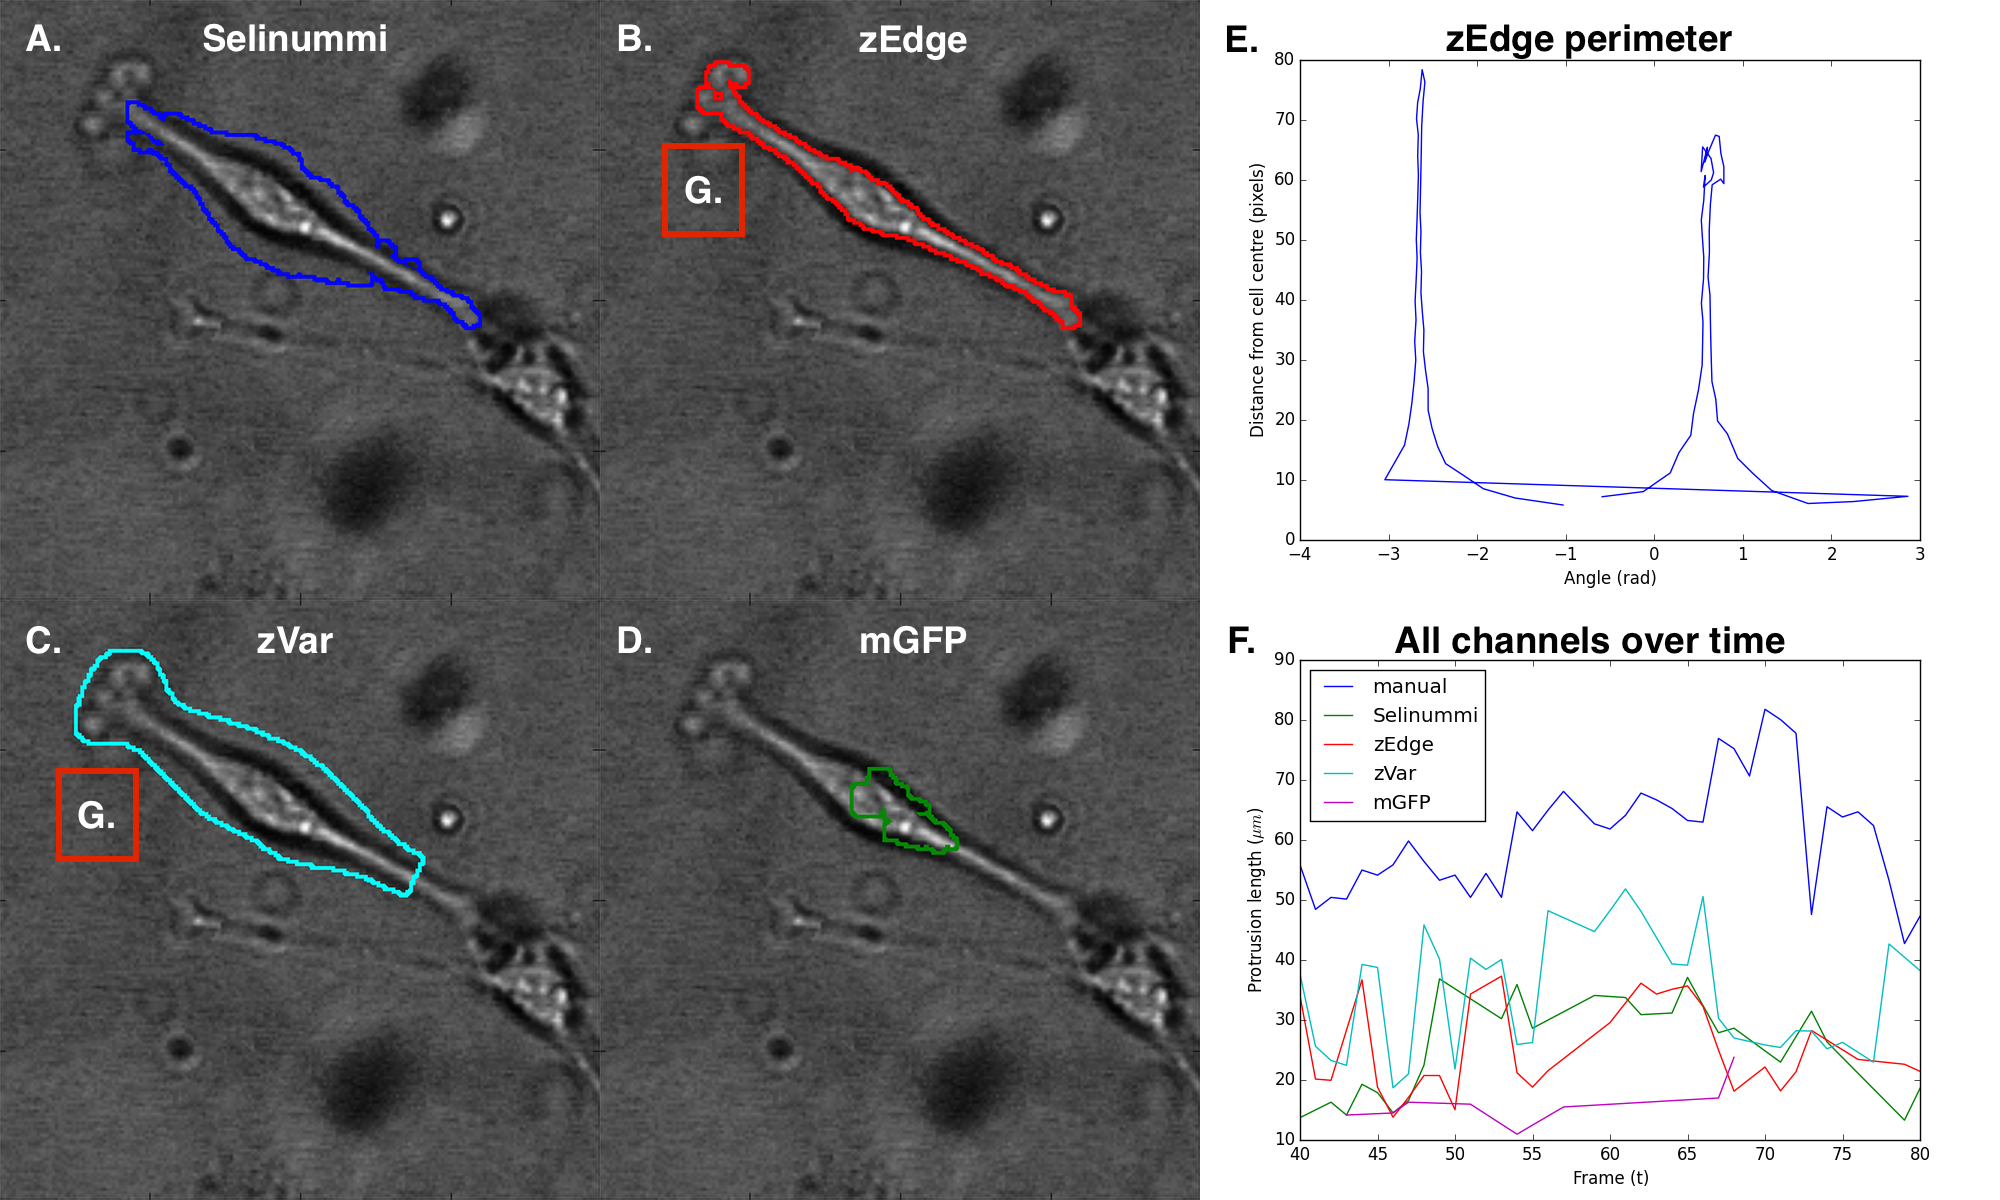
\includegraphics[width=0.9\textwidth]{510_protrusion_comparison}
 \caption[Testing: protrusion comparison]{
	Cell masks can also be compared by how well the extremities of the cell are segmented. ABCD show four different masks of the same cell from four different channels (Selinummi, zEdge, zVar, and mGFP (the maximum GFP projection) respectively). By tracing a line around the perimeter of the shape, a distribution similar to that shown in E can be found for each cell; an ordered list of distance against angle around the centre point. This can then be used to find any peaks that diverge from the mean radius. These can be classed as protrusions and their lengths and orientations found. A comparison based on complex shape features is hard to compress into one or two values such as in Figure~\ref{fig:areacomparisonvalues}. For example, the protrusion on the left, marked G, is longer in the zVar (C) channel than in the zEdge (B) channel, but the zEdge segmentation of the protrusion is closer to the overall shape. Most protrusion lengths will fall short of the true length as segmented manually. This type of analysis is not current quantifiable, but it can be investigated using this method of image pre-processing.
 }
 \label{fig:protrusioncomparison}
\end{figure}

\section{Errors and limitations}
\label{sec:errors}

Several possible errors that would affect segmentation results must be mentioned for completeness. Some of these error have not been observed, but are possible given certain conditions. Errors can be caused by faults in the microscope hardware, irregularities in the illumination of the environment for any reason, poor choices in imaging setup, or particular configurations of cells that cause the method to fail.

A controversial example of a possible error is a situation where two cells are superimposed in Z. In this case, a GFP profile for a single XY location could have two very prominent peaks. Currently, the method does not attempt to resolve this situation since it has not been observed in the current data, but trivially, it could be resolved by only taking account of the peak with the highest Z level, since the brightfield information is not 3D, and there is no way to recover any edge information about the lower cell if it is obscured. In this case, such a conflict could be noted and the GFP edge, which is not obscured, could act as a fallback for the segmentation. This information would allow the GFP edges, while they are suboptimal, to be incorporated into the outline of the rest of the cell if it is visible elsewhere in the brightfield. To reiterate, this situation has not been observed, but it is theoretically possible in such a 3D environment. A hypothetical example can be seen in Figure~\ref{fig:superimposedcells}.

\begin{figure}[h!]
 \centering
 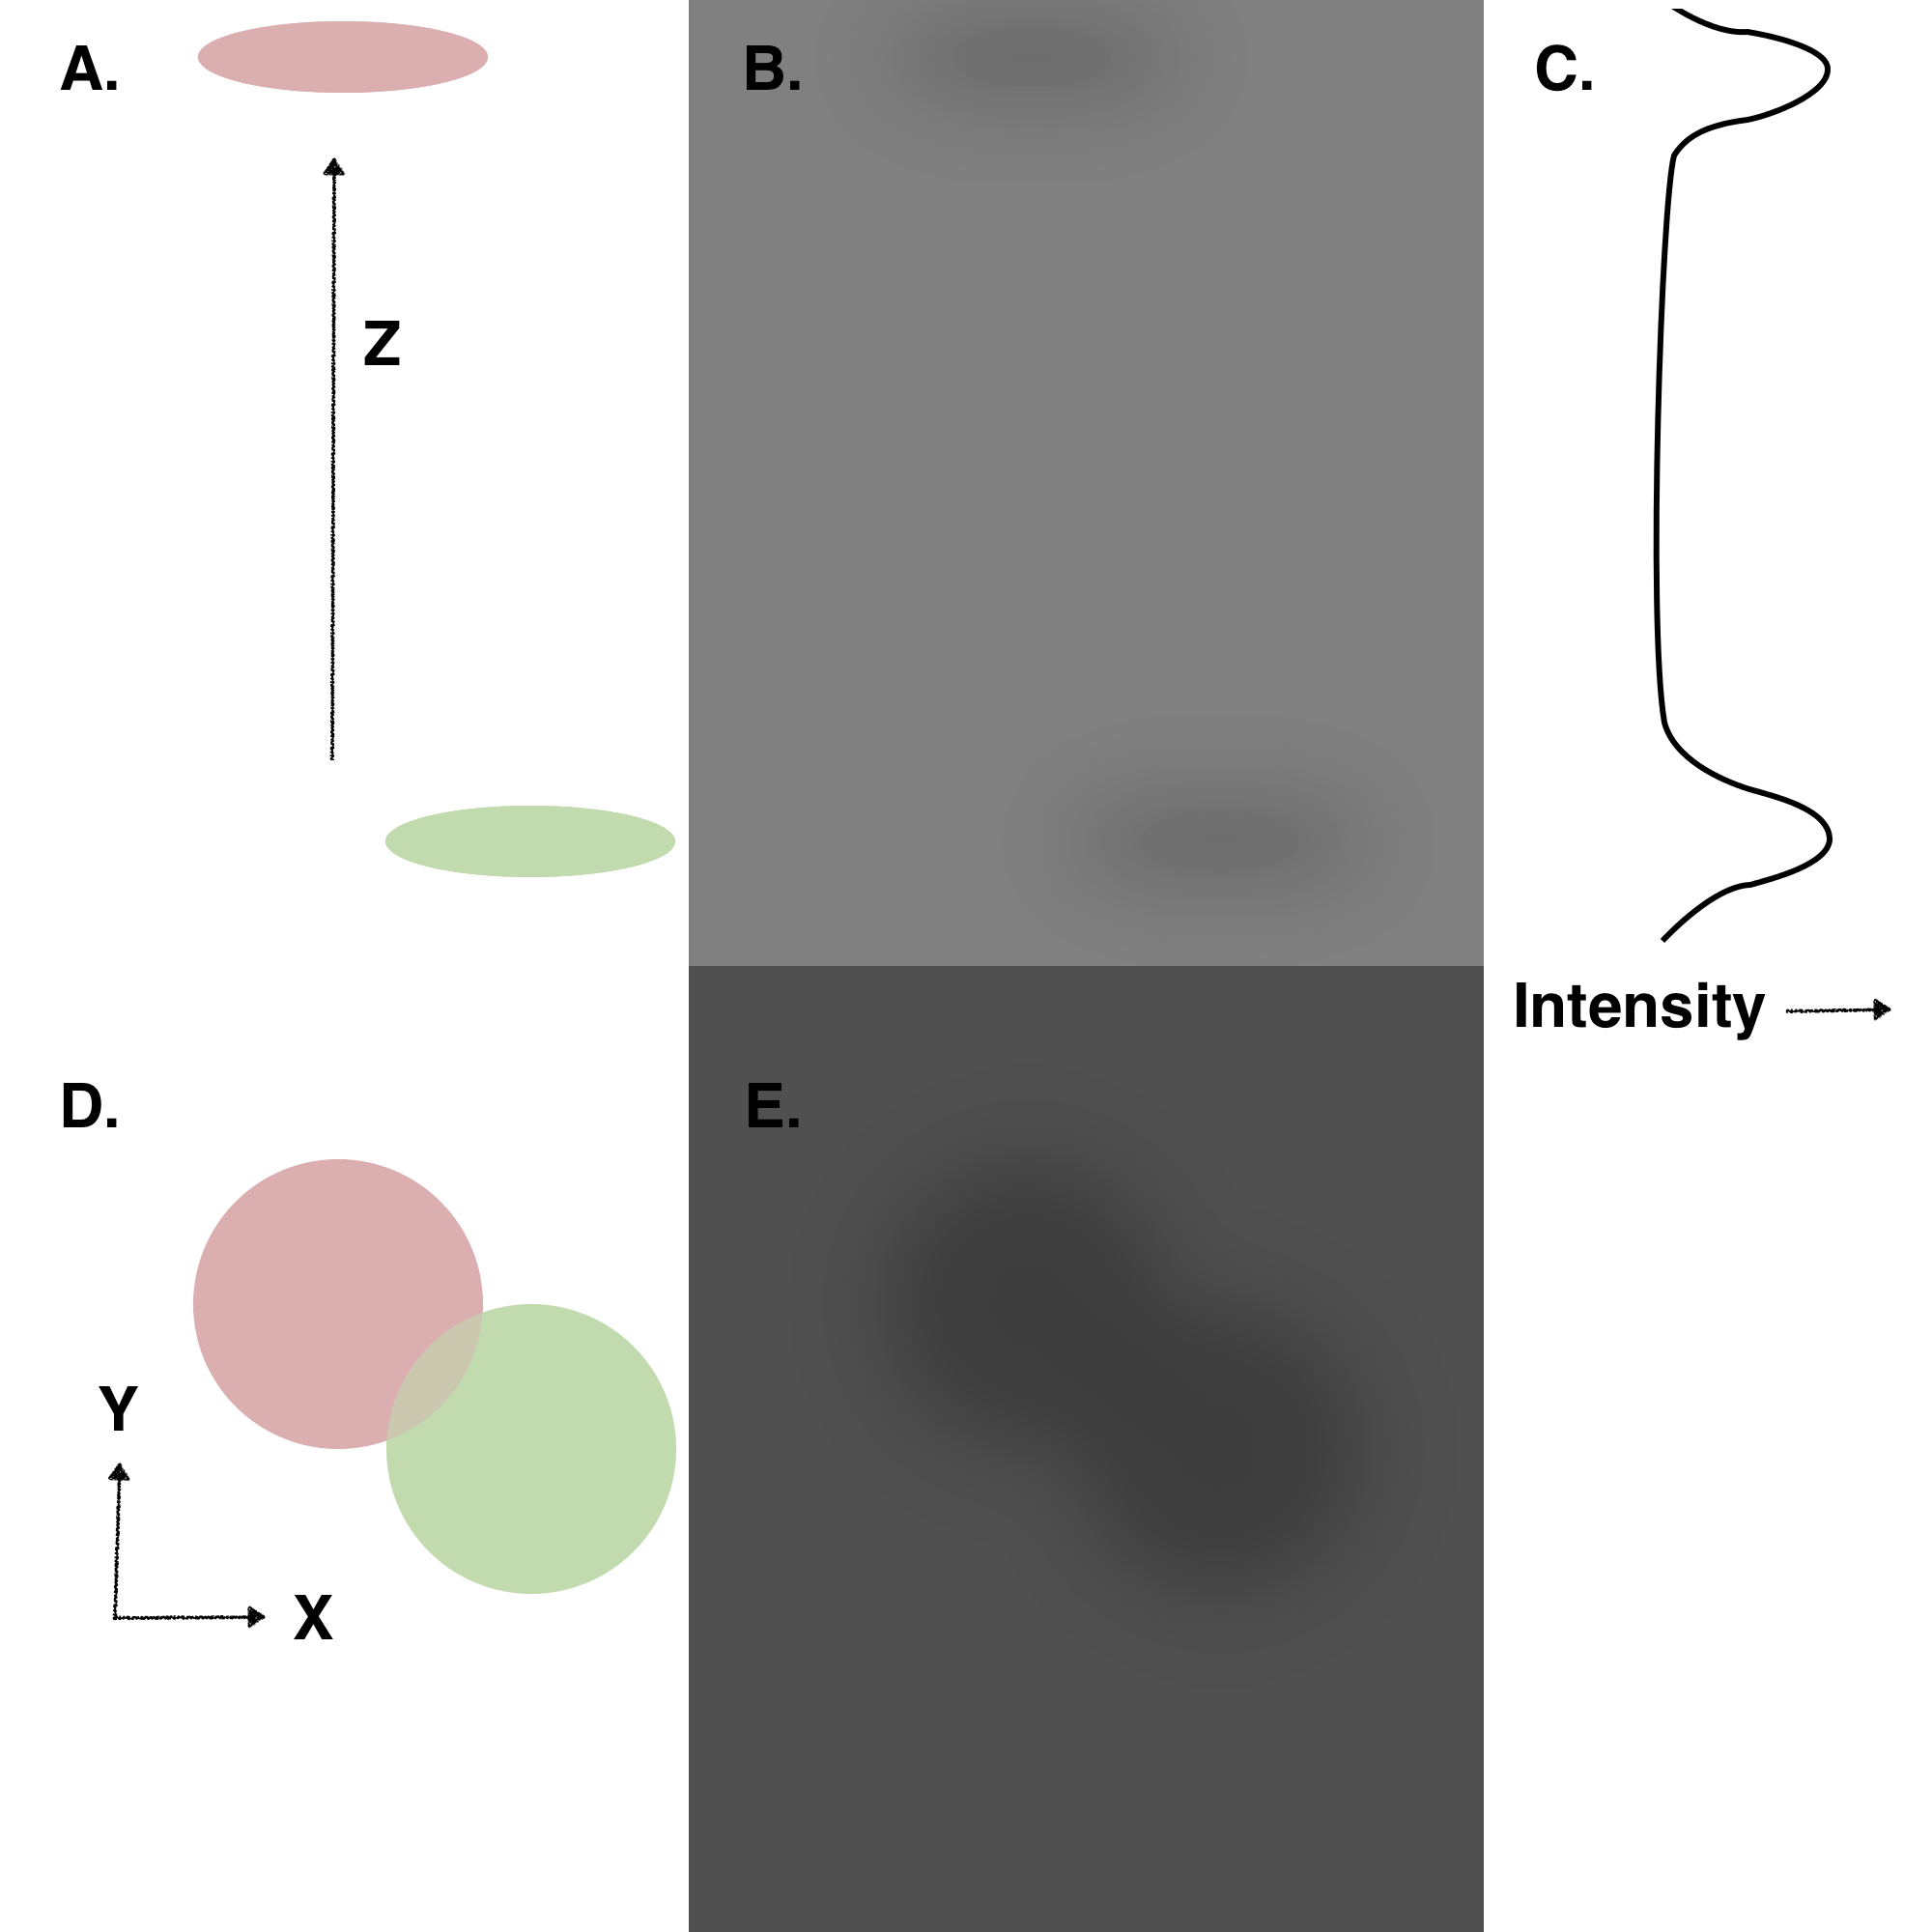
\includegraphics[width=0.9\textwidth]{511_hypothetical_superimposed_cells}
 \caption[Unaccounted for: superimposed cells]{
 	A potential weakness of this method is a situation which has not been fully encountered. If two cells lie superimposed at very different levels in the environment, as depicted in A, it is possible that there will be two distinct peaks in Z as shown in C. In this situation, the current algorithm would take the maximum peak as the value to be added to zMod. If the cell with the greater value is the lower one, the brightfield representation would not be complete. The brightfield information between different levels in mixed and can only be seen from above. The cell above would be the most useful candidate to level-correct. This situation has not been encountered in the current data, and the method would have to be modified to account for this possibility.
 }
 \label{fig:superimposedcells}
\end{figure}

In some cases, through a hardware fault or a temporary shift in the illumination of the environment, the level of the GFP intensity can drop in the whole experiment. This happened in one experiment done and caused the method to fail in a single frame, and subsequently rendered the area estimates in that frame for all objects unreliable. This effect can be seen in Figure~\ref{fig:lowgfpillumination}.

\begin{figure}[h!]
 \centering
 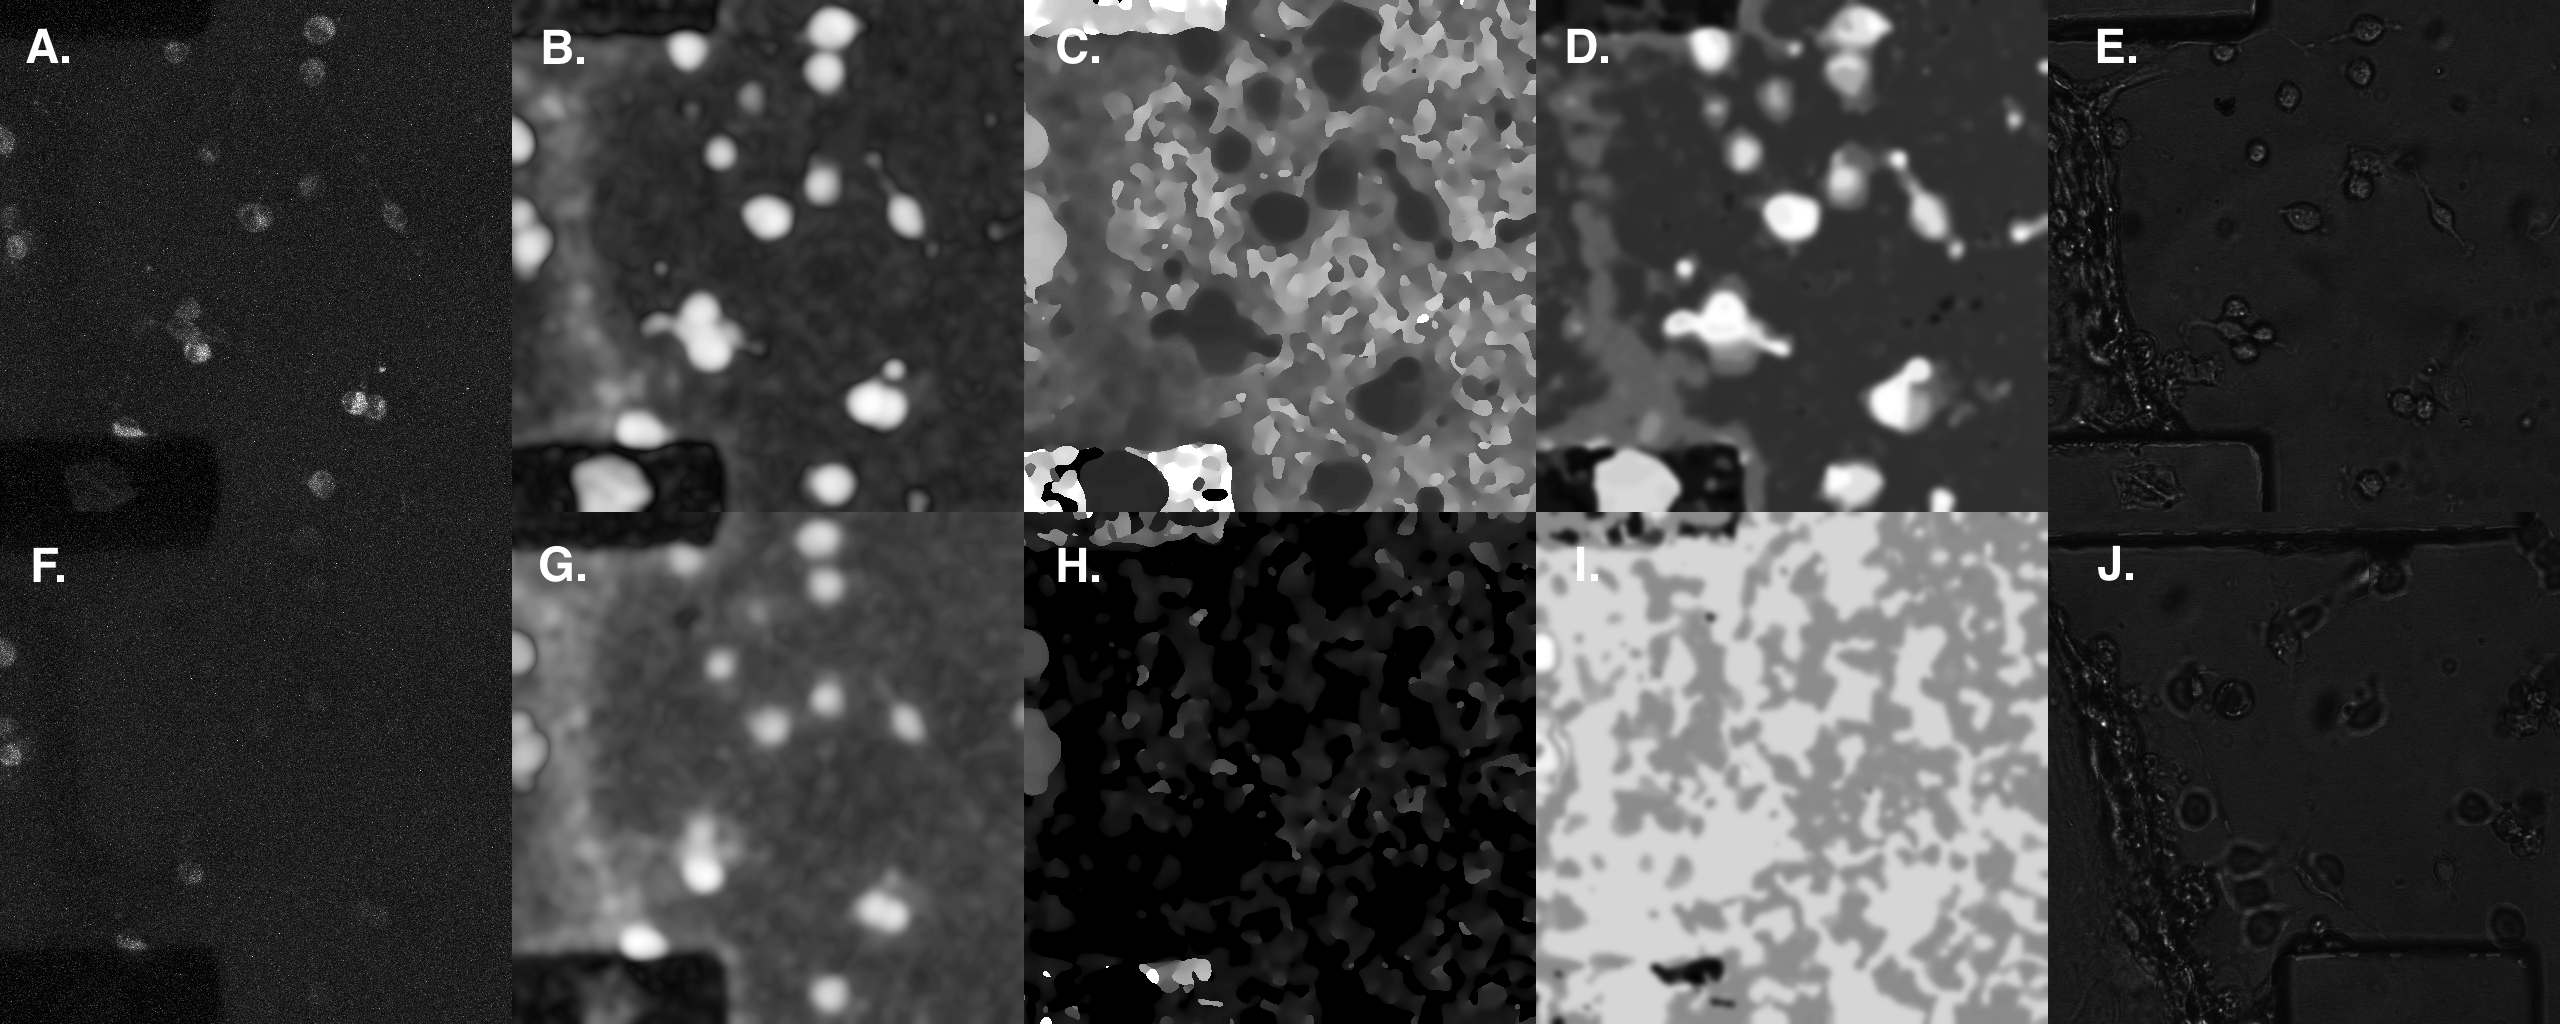
\includegraphics[width=0.9\textwidth]{512_low_gfp_illumination}
 \caption[Effects of low GFP illumination]{
 	As stated before in Figure~\ref{fig:lowgfp}, this method does not work in low GFP conditions. From left to right, the images are A, The GFP Z projection; B, the zVar image; C, the zMod image; D, the zUnique image; and E, the zBF image. ABCDE shows the method under normal GFP conditions. FGHIJ shows the environment one frame later when the illumination has dropped significantly. Note particularly A compared to F. There is very little GFP present. In contrast, the variance image, zVar, still shows a strong response, a testament to the utility of this information. zMod suffers from the drop in GFP lacking a consistent Z location within cells. Similarly, the zUnique contrast drops. The result is an incorrectly level-corrected image in zBF.
 }
 \label{fig:lowgfpillumination}
\end{figure}

If the illumination of the environment is not uniform, and regions at the top are significantly brighter than the bottom for example, when brightfield pixel values from different Z levels are brought together to generate zBF, it is possible that the intensities are so different as to be discontinuous, leading to the appearance of a false edge. This type of effect is shown in Figure~\ref{fig:crosslevelartefacts}. This can be alleviated partially by the choice of $R$ or $\Sigma$, since both control to a certain extent the smoothing between levels. If transitions between levels are smoother, artefacts such as these are less likely to form.

\begin{figure}[h!]
 \centering
 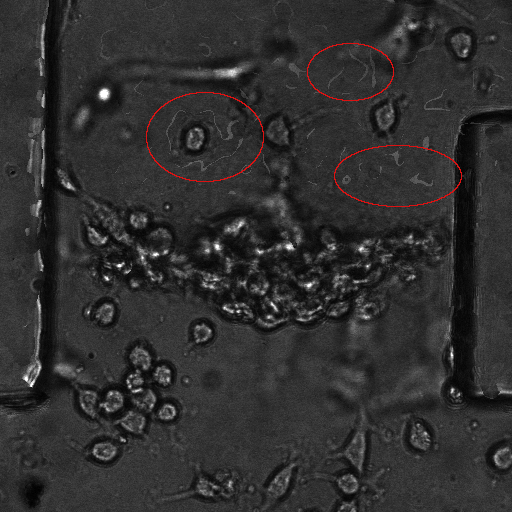
\includegraphics[width=0.9\textwidth]{513_cross_level_artefacts}
 \caption[Cross-level artefacts]{
 	zBF is created by taking brightfield values from all different parts of the image stack. It is possible that illumination at the top and bottom of the stack may differ, sometimes significantly. In this case, darker pixels may be placed in the zBF image adjacent to light pixels from another level. This results in a mottled appearance of the zBF image. The highlighted boxes contain features that could be interpreted as objects or parts of objects by a recogniser. This is possible a weakness. Improved smoothing methods and gradual object recognition could solve this problem. This means segmentation carried out at each stage of the image modification process could be combined to decrease error at the final stage.
 }
 \label{fig:crosslevelartefacts}
\end{figure}

Finally, if the configuration of the microscope is chosen before imaging to yield generally low contrast brightfield images, edges may not be visible in any focal plane. In this case, the method of finding the in-focus representations of cells may not be very useful as no more information is revealed. In this case, an alternative might be use the segmentation of the GFP primarily and gather what results are available from the brightfield. As with hypothetical superimposed cells, edges from GFP and brightfield channels could be combined, but here it might be more effective to weight the edges found in GFP to be more reliable than those in the brightfield. This is subject for future work.

\begin{figure}[h!]
 \centering
 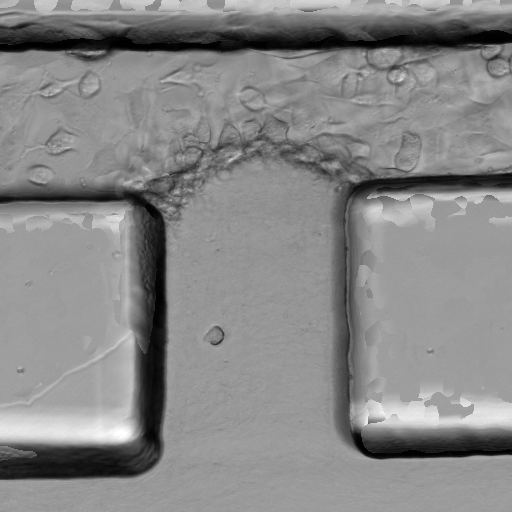
\includegraphics[width=0.9\textwidth]{514_no_bf_contrast}
 \caption[Lack of brightfield contrast]{
 	Low GFP intensity is very harmful to this method, but even if the GFP is very high contrast with low noise, a lack of brightfield contrast can also prevent the method from working. If the brightfield has low contrast, then edges of cells and other objects will not be as visible. Even if the images are level corrected properly, there might not be enough information to segment the cells properly. Shown is an example of an experiment with very poor contrast in the brightfield. This cannot be solved numerically and must be carefully adjusted in the microscope prior to imaging.
 }
 \label{fig:nobfcontrast}
\end{figure}
